\chapter{Hardware and Software Activities}
\label{chap:Hardware}

The Hadron Outer (HO) calorimeter of the CMS detector has been installed to measure the energy which is not contained by the barrel calorimeters. The HO improves the energy resolution of highly energetic hadrons and hence provide a better jet energy reconstruction as well as missing transverse energy resolution. HO is situated in the barrel return yokes (YB) in front of the first layer of muon chambers. The YBs consist of 5 rings of iron: YB0, YB$\pm$1 and YB$\pm$2. Rings R0, R$\pm$1 and R$\pm$2 of the HO system are located in YB0, YB$\pm$1 and YB$\pm$2 respectively. In the original design of HO, the signals of the detector were read out by hybrid photo-diodes (HPDs) by converting the wavelength shifted scintillator light into electrical charges. The electronics readout system of the HO is built using the 18-channel readout modules (RMs). The RMs combine the photo-sensors, amplifiers and analogue to digital converters (ADC) and are housed in crates (RBX). The newly developed SiPM system consists of three circuit boards : a mounting Board (MB) holding the SiPM, a bias
board generating the SiPM operation voltage and the Control Board (CB). 


onsists of a stack of three printed circuit boards: a mounting board
holding the SiPM and a Peltier element for active temperature control of the SiPM, a bias
board generating the SiPM operation voltage, and a control board that regulates and monitors
the operation of the individual SiPMs as well as the Peltier element. The control board also
connects the SiPMs electrically to the HCAL readout electronics. 

The array of 18 SiPMs is mounted on one side of the MB. The geometrical constraints required a total of 132 RMs to read all channels. The HPDs were chosen as photo-sensors due to its high gain and magnetic field tolerance. But in Run I conditions of the CMS, HPDs proved to be less optimal because of the discharge caused by the fringe field of the CMS magnet, low gain and photo detection efficiency, and ageing effects. Due to these inefficiencies, the HPDs needed to be replaced with multi-pixel Geiger-mode avalanche photo-diodes also known as silicon photo-multipliers (SiPMs). The SiPMs are preferred because of the magnetic field insensitivity, relatively high gain and high photon-detection efficiency. This replacement was carried out during the first LHC long shutdown (LS1) in 2013-2014 \cite{Lutz:2012yoa}, where the LHC was upgraded to higher luminosity (5 $\times$ 10$^{34} {\rm cm}^2 {\rm s}^{-1}$) and center-of-mass energy of proton-proton collisions was increased from 4 TeV to 6.5 TeV per beam. During this up-gradation, the replacement of HPDs took place in two steps : first the existing RMs with HPDs were taken out from the detector and then were rebuild with SiPMs. After verifying the working of the RMs, they were re-installed in the CMS detector. In collaboration with HO group of the CMS, we participated in the re-installation of the RMs with SiPMs in place of HPDs specially in the sectors YB\plusn 1 and YB\plusn 2 of HCAL during the visits to CERN in March-April, 2014.

\section{Silicon Photo-Multipliers}
A silicon photo-multiplier (SiPM) used in HO is a Hamamatsu Multi-Pixel Photon Counter (MPPC) in a surface mounted device housing. It has a cell pitch of 50 $\micro$m with an active area of 3 $\times$ 3 mm. The required operating voltage required is $\sim$ 70 V with a gain $\sim$ 6 $\times$ 10$^5$ fC/photo-electron when operated at a voltage greater than the breakdown voltage by 1 V. At this over-voltage given by the bias voltage subtracted from the breakdown voltage, the typical dark current rate is of the order of a few hundred kHz. Along with the installation of SiPMs, the commissioning of the upgraded parts also took place. The commissioning includes the quickly identification of the problems with the new and existing hardware, validation of the installation and repairs, in case of any malfunctions, during the access to the hardware. To monitor and optimize the operational parameters, two types of data were used : the signals from SiPMs in the absence of light referred as pedestal events (PED) and the charge distributions collected by illuminating the SiPMs with a calibrated light emitting diodes referred as LED events. While performing the Quality Control (QC) analysis, the PED and LED events or runs were taken through an online software created by HO CMS group. These runs were used to study and analyze the properties of SiPMs. 

In the first step of commissioning, a communication test was performed with the readout system along with the verification of slow control operation and channel response. After that, the measurements and optimization of SiPM operational variables were carried out. One of the important quantities of the SiPMs to study is the change of breakdown volatge (BV) and calibration factor gain (G) with the temperature. BV
gives the threshold voltage after which the diodes switch to avalanche mode and gain corresponds to the charge produced by SiPM for a single photo-electron (SPE). The gain of SiPMs depends linearly on the temperature with a relative dependence of 8\% gain shift per K at an operating point of 1.5 V over-voltage \cite{Anderson:2011zzc}. As the gain depends linearly on the over-voltage, the change of the breakdown voltage with temperature translates into a change of the gain with temperature. This dependence requires an active control of the temperature of SiPMs with better than 0.1 K stability. So a peltier element is mounted on the back of the MB for cooling purposes in order to stabilize the temperature. We mainly studied the variations of BV and gain with temperature : \\ \newline

{\bf Breakdown Volatge (BV) -}

Once operating temperature is adjusted and system is thermally stable, the breakdown temperature is measured using methods described
in Sections 3.1.1 such that target gain for all channels is ∼ 6 ADC/photo-electron to
prevent the ADC from saturation, but still have a good signal-to-noise ratio.
After the successful completion of these commissioning steps, the new readout hardware is
ready for data taking.




For the determination of the breakdown voltage, there is also the possibility to use either the
pedestal spectrum of the SiPM or the signal of a short LED pulse. For the first method the gain
is determined for different applied bias voltages. The gain depends linearly on the operating
voltage so the resulting curve is a straight line which can be extrapolated to gain 0 as is shown

in Fig. 7. At the corresponding bias voltage the breakdown of a cell is just about to start
which is the definition of the breakdown voltage. The second way is to use the relative change
of the measured signal when pulsing an LED and varying the bias voltage. As shown in Fig.
dS
8 the distribution of SdV
peaks at that voltage, at which the change of the relative signal is at
maximum which is then used as the breakdown voltage. The distribution of the variation in

breakdown voltage over time for one PCB using the LED method is shown in Fig. 9. The time
period reaches from the end of January to the beginning of March in 2014. The breakdown
voltage is found to be stable within 50 mV which demonstrates the reliability of the breakdown
voltage determination. For comparison with the pedestal method refer to section 4.2.

\begin{figure}[!h]
\begin{center}
\vspace*{3mm} 
\hspace*{-5mm}
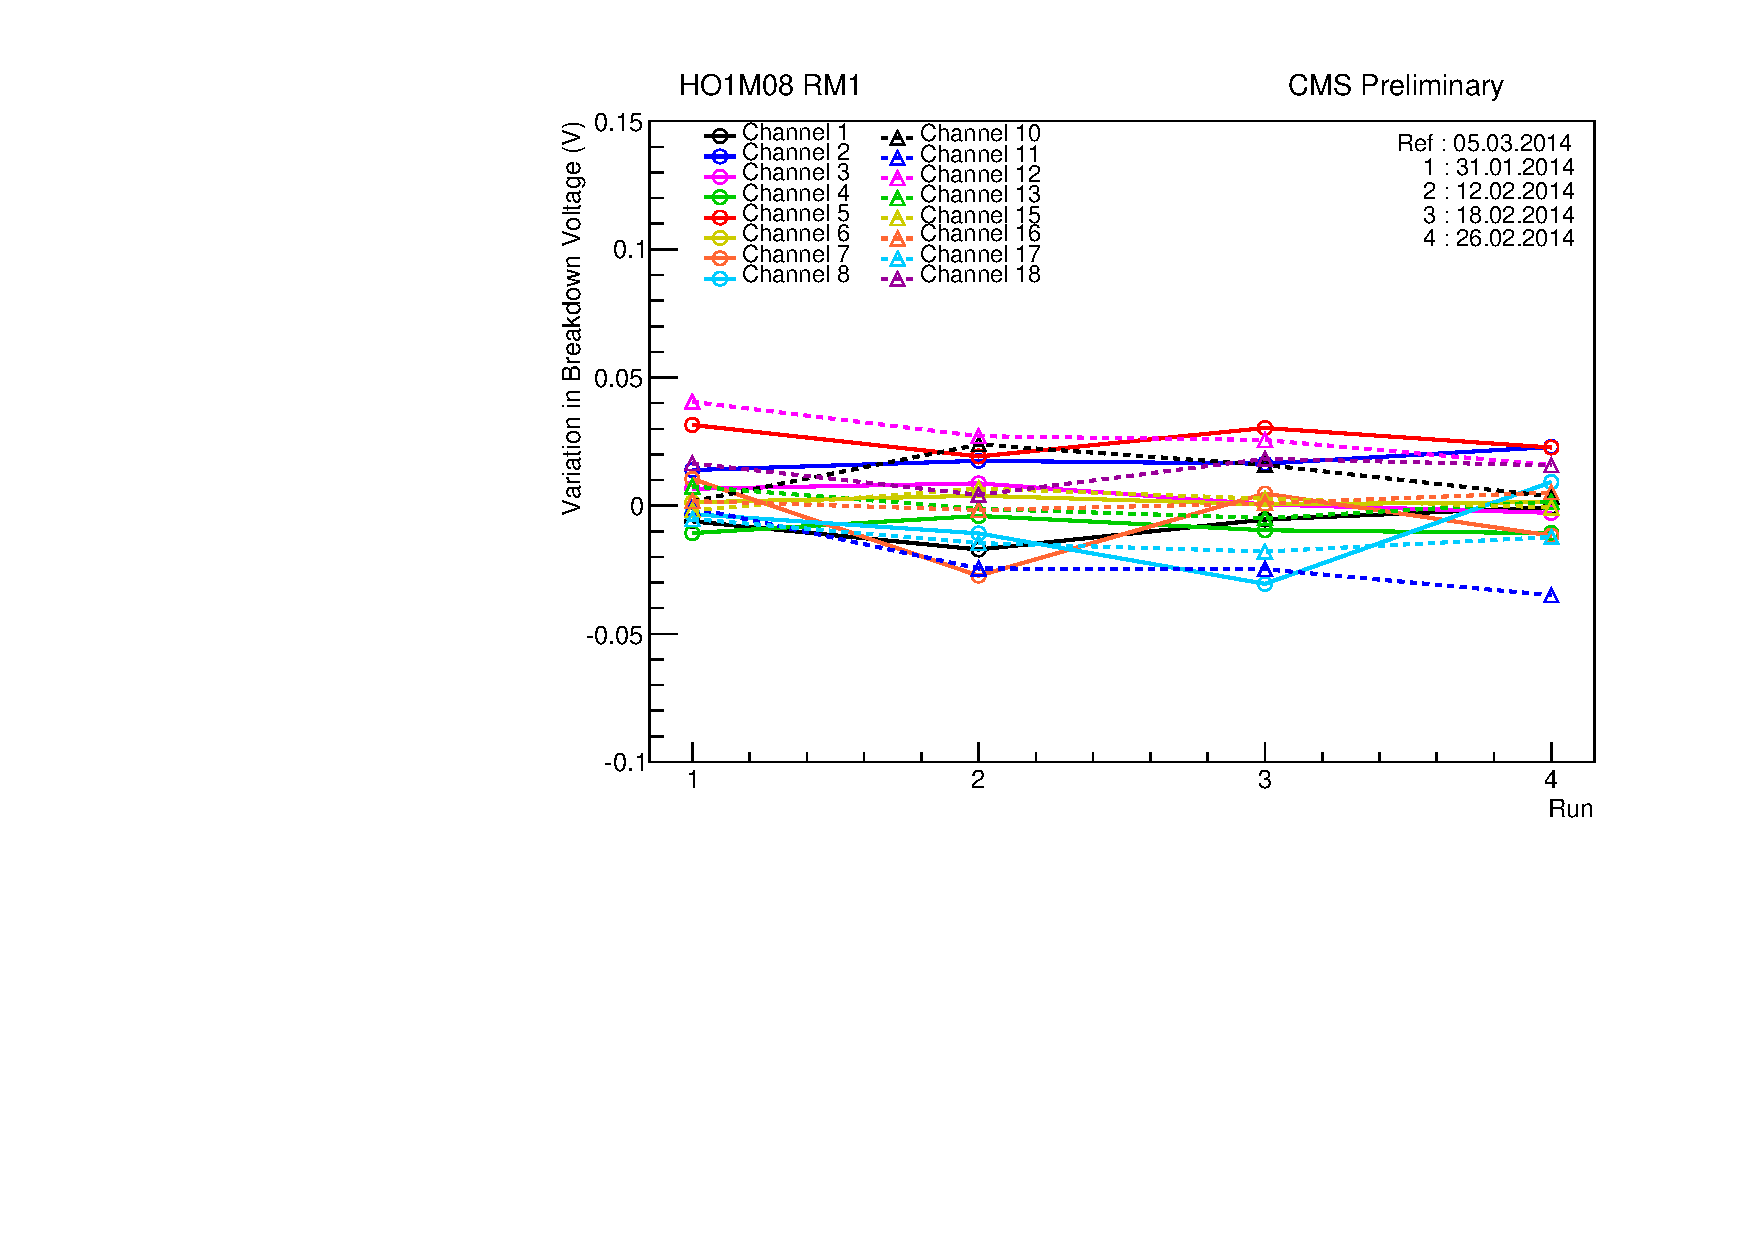
\includegraphics[scale = 0.65]{/home/anter/Desktop/Thesis/Figures/Final/bv_led_iv_49.pdf}\\
\vspace*{4mm}
\caption{Distribution of the
breakdown voltage over time for one
PCB (18 channels)}
\label{fig:BV}
\end{center}
\end{figure}



When detector is operated in stable conditions we find the BV measurements also stay stable
within 50 mV, as shown on Fig. 10, which demonstrate the reliability of the breakdown voltage
determination. Variation of gain is also monitored over period of time and it is found to be
within 3% for all SiPMs, see Fig. 11. This demonstrates that the gain determination works as
expected and the operation of the SiPMs with a stable gain is possible.

\begin{figure}[!h]
\begin{center}
\vspace*{3mm} 
\hspace*{-5mm}
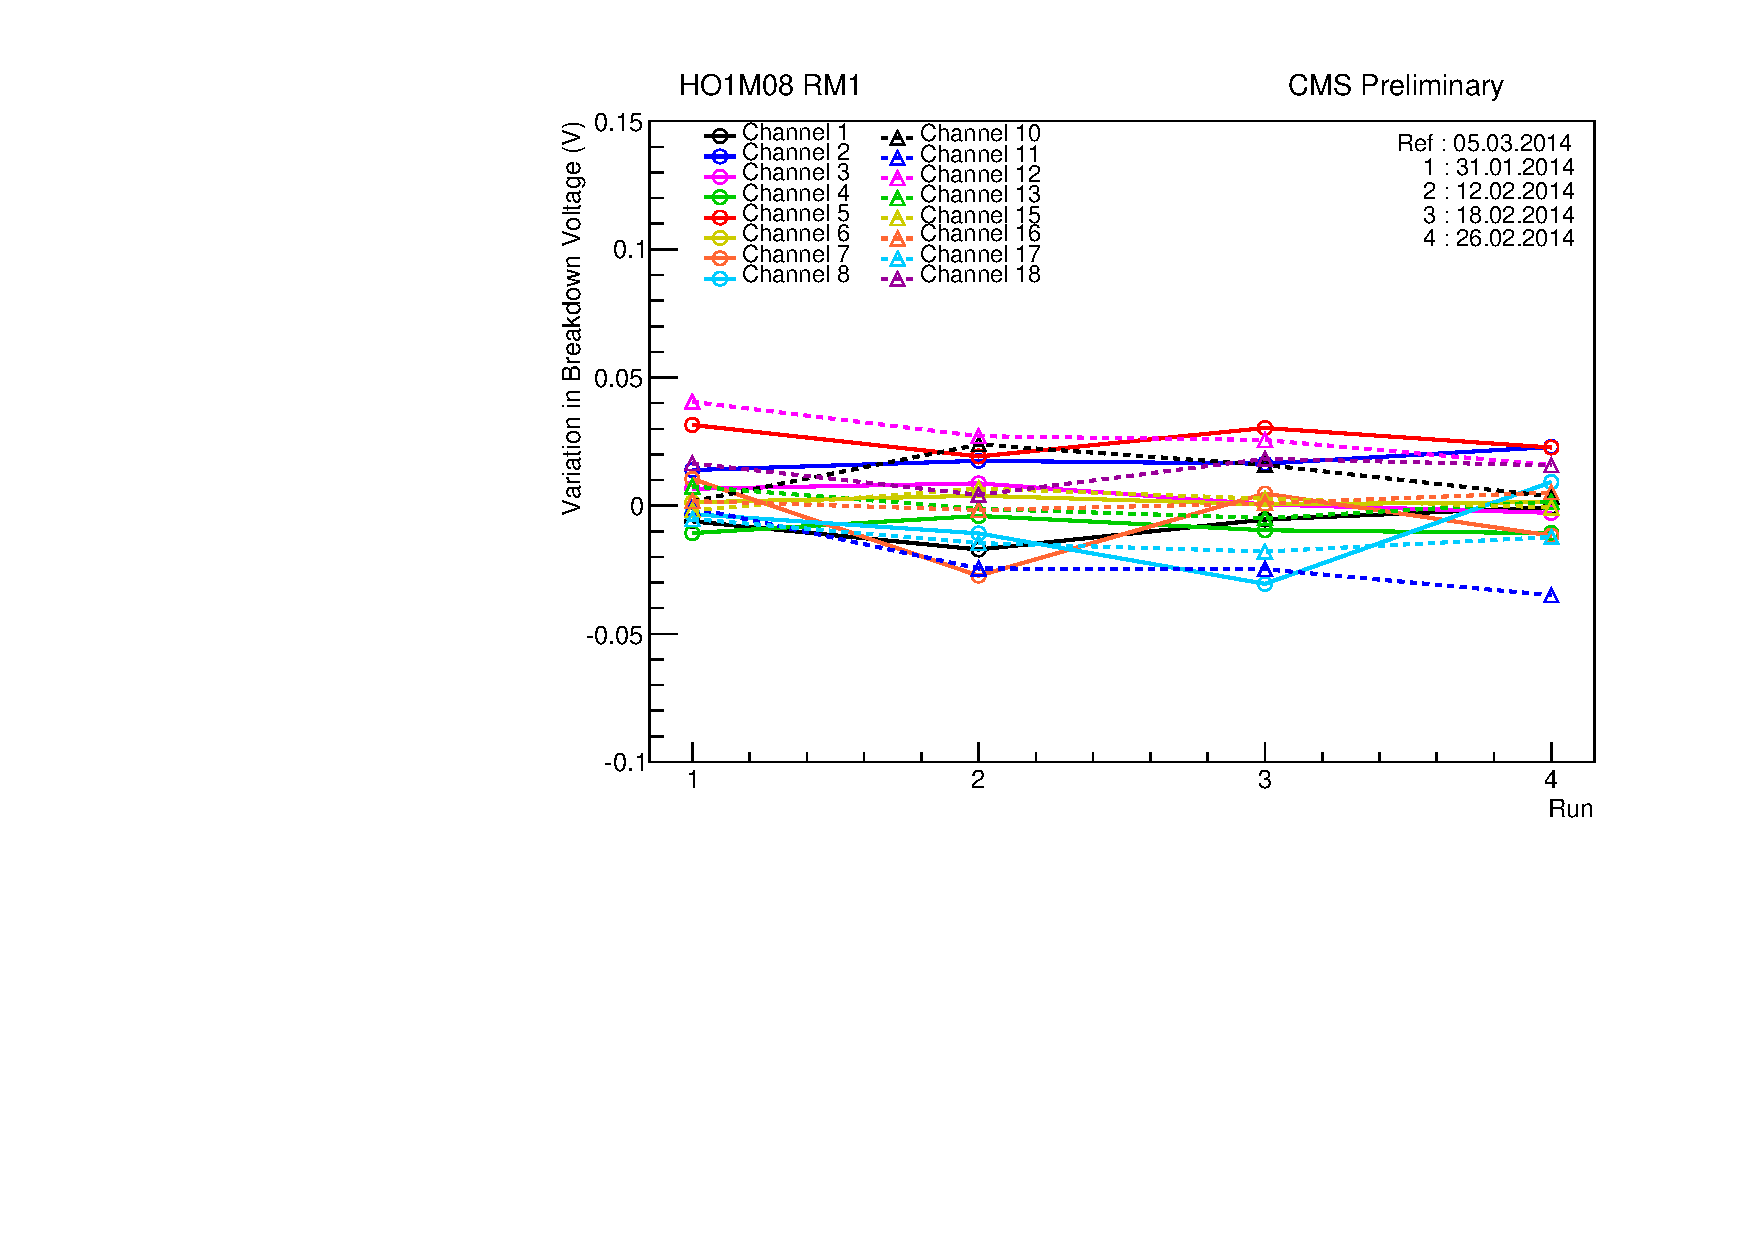
\includegraphics[scale = 0.65]{/home/anter/Desktop/Thesis/Figures/Final/bv_led_iv_49.pdf}\\
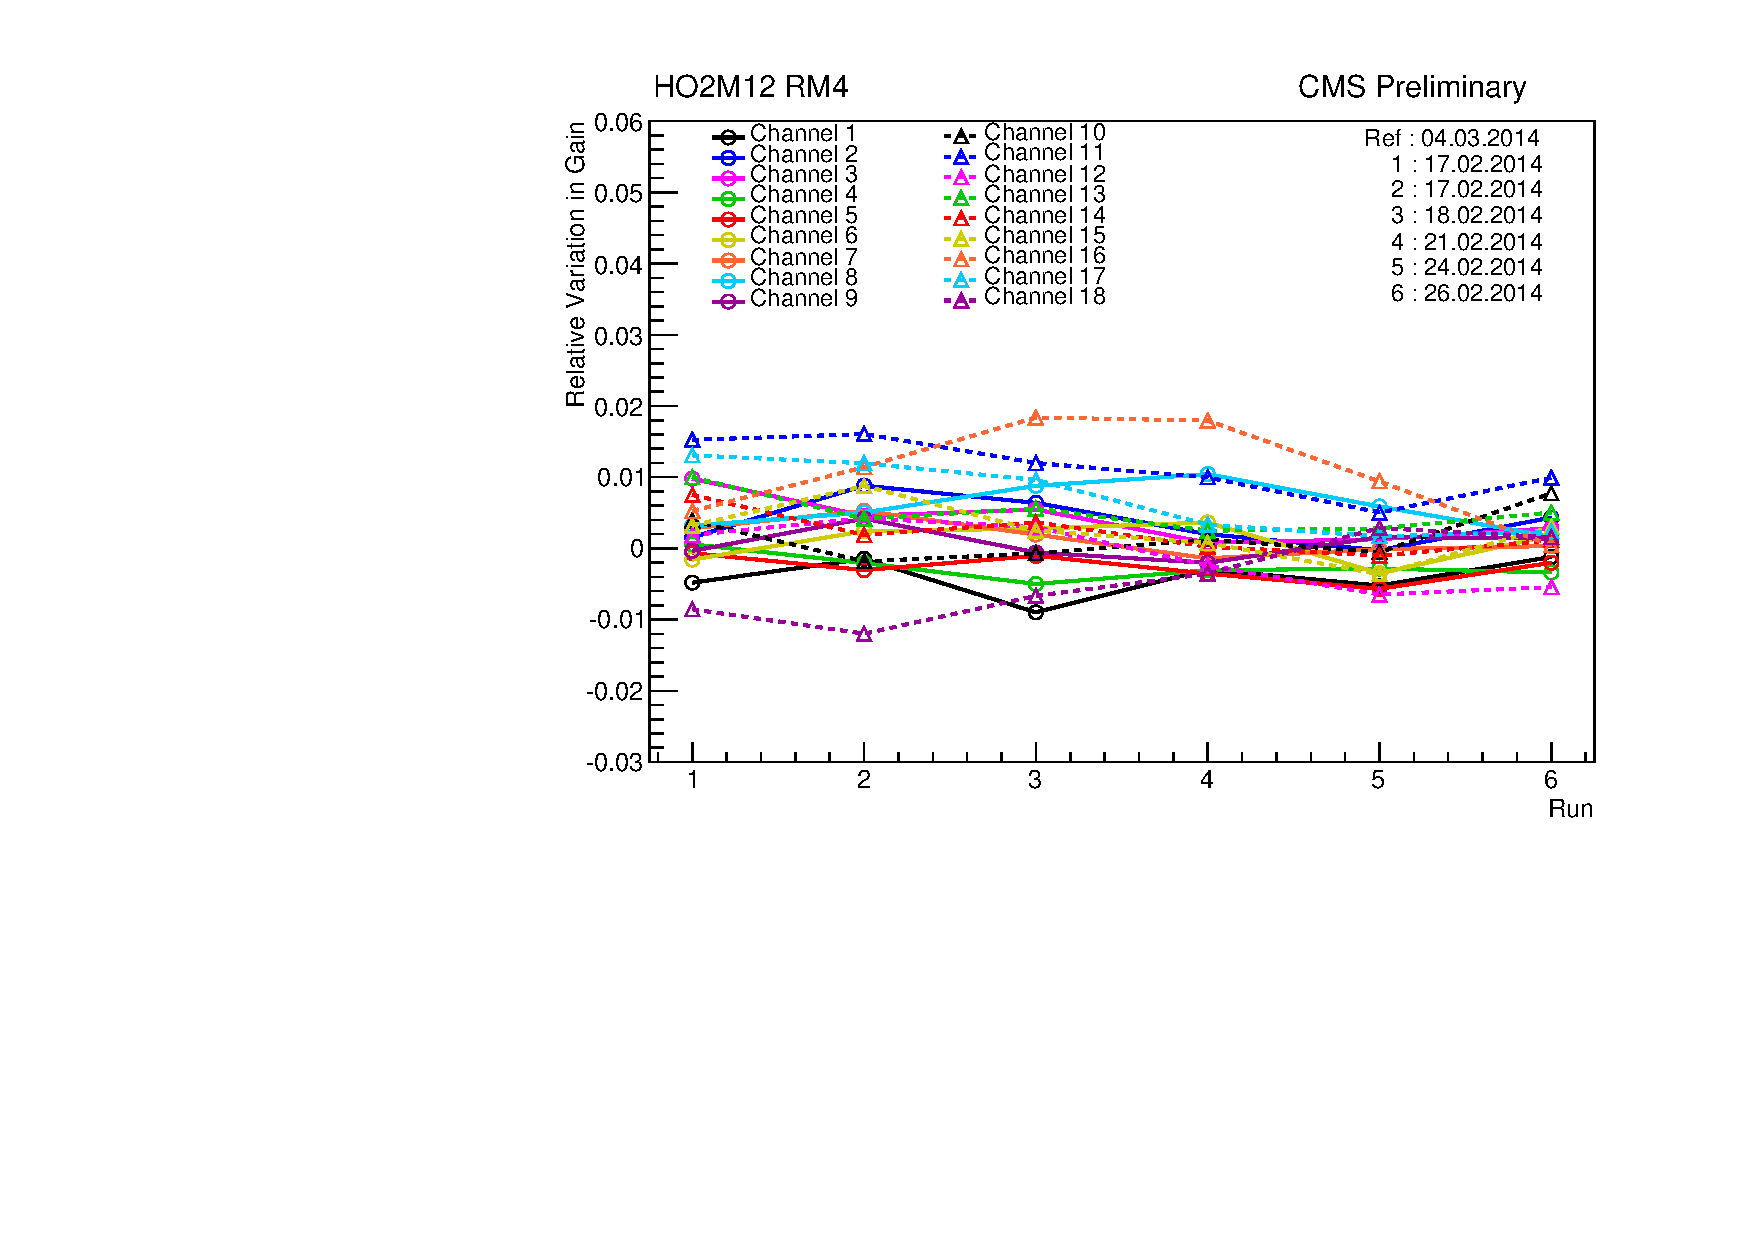
\includegraphics[scale = 0.65]{/home/anter/Desktop/Thesis/Figures/Final/Gain_PED_108.pdf}\\
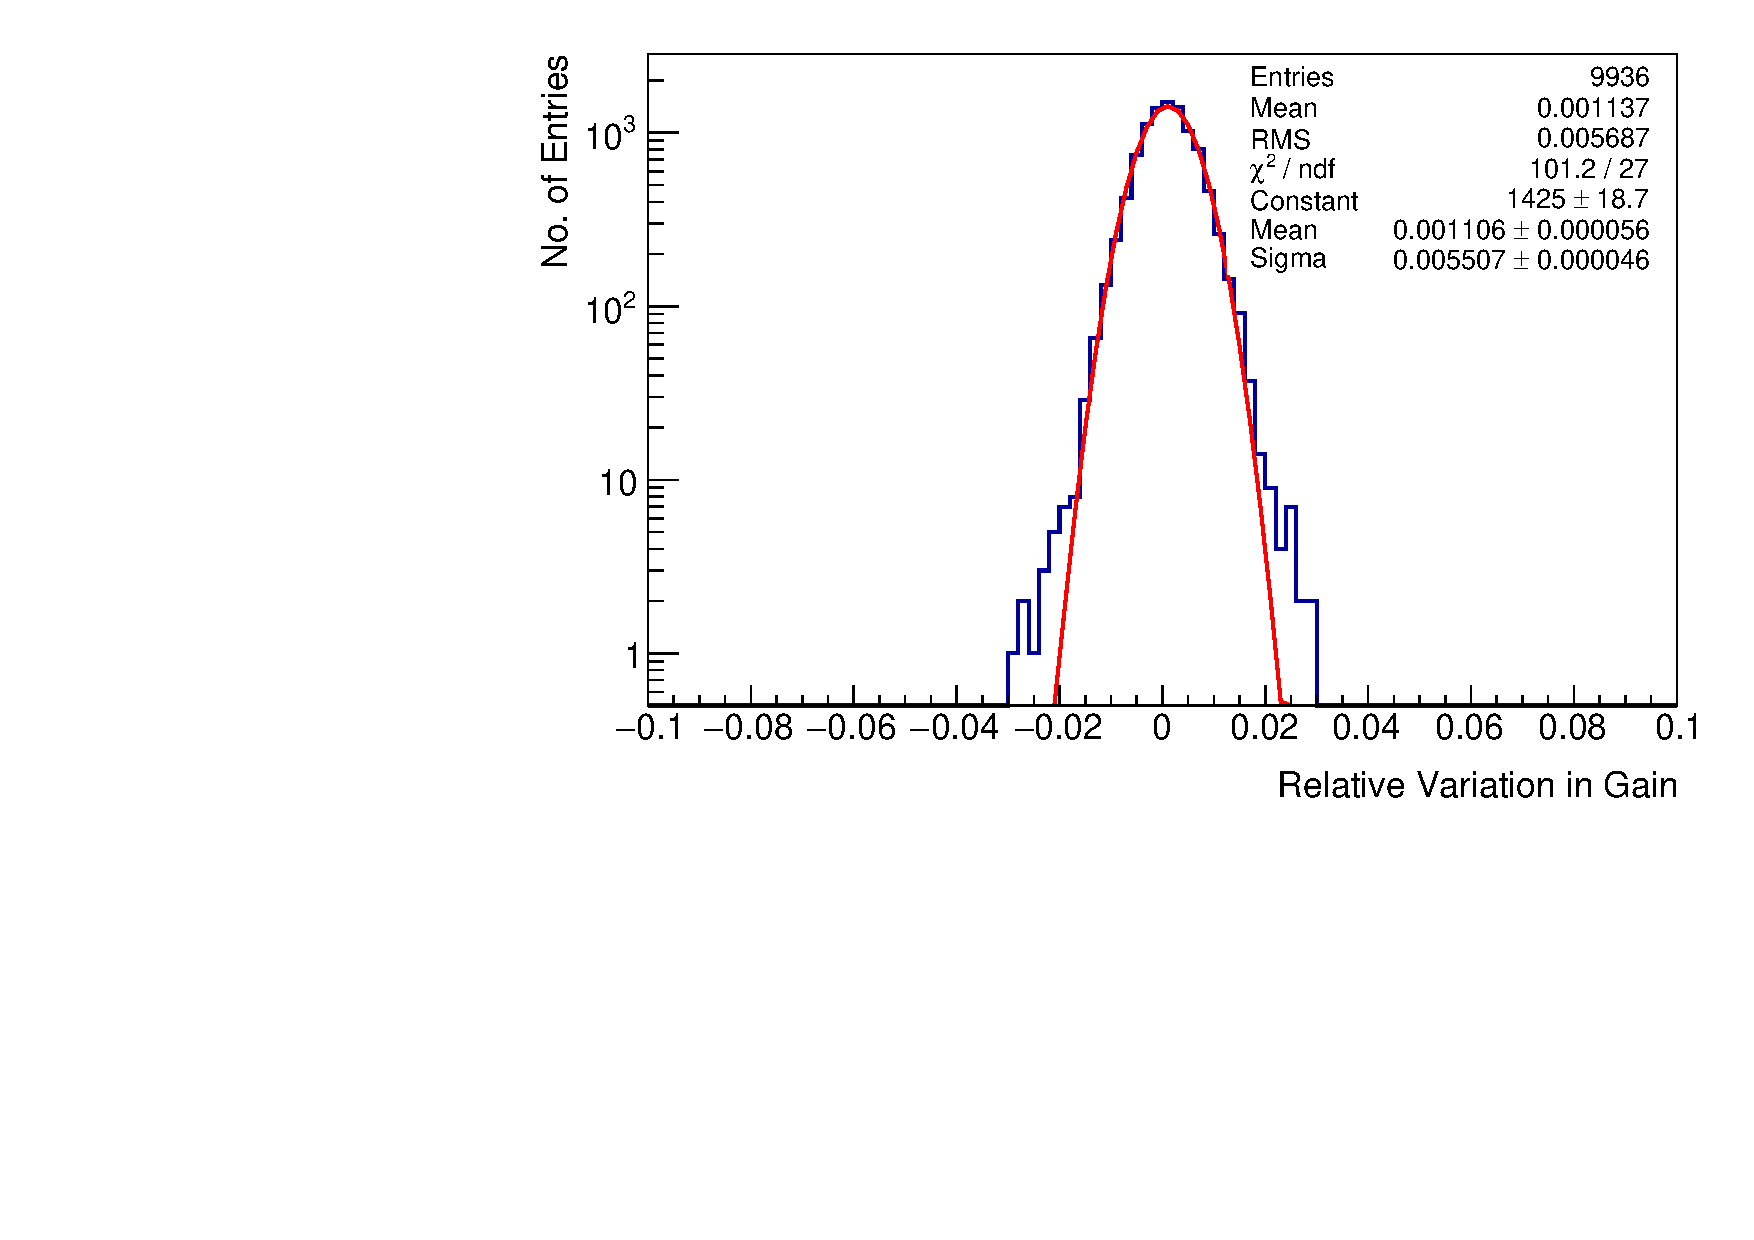
\includegraphics[scale = 0.6]{/home/anter/Desktop/Thesis/Figures/Final/Fit.pdf}
\vspace*{4mm}
\caption[Longitudinal section of one quarter of the hadronic calorimeter (HCAL) in $r$-$\eta$ plane.]{Longitudinal section of one quarter of the hadronic calorimincludegeter (HCAL) in $r$-$\eta$ plane. It consists of different parts : hadron barrel (HB), hadron outer (HO), hadron endcap (HE) and hadron forward (HF). Taken from \cite{Chatrchyan:2008aa}.}
\label{fig:hcal}
\end{center}
\end{figure}

These results were presented at the CALOR2014
conference [110], and documented in Ref. [113]

\cite{Kunsken:2015zla}
{\bf Mtca importance : pics}

{\bf Data Certification}




\begin{figure}[!h]
\begin{center}
\vspace*{3mm} 
\hspace*{-5mm}
%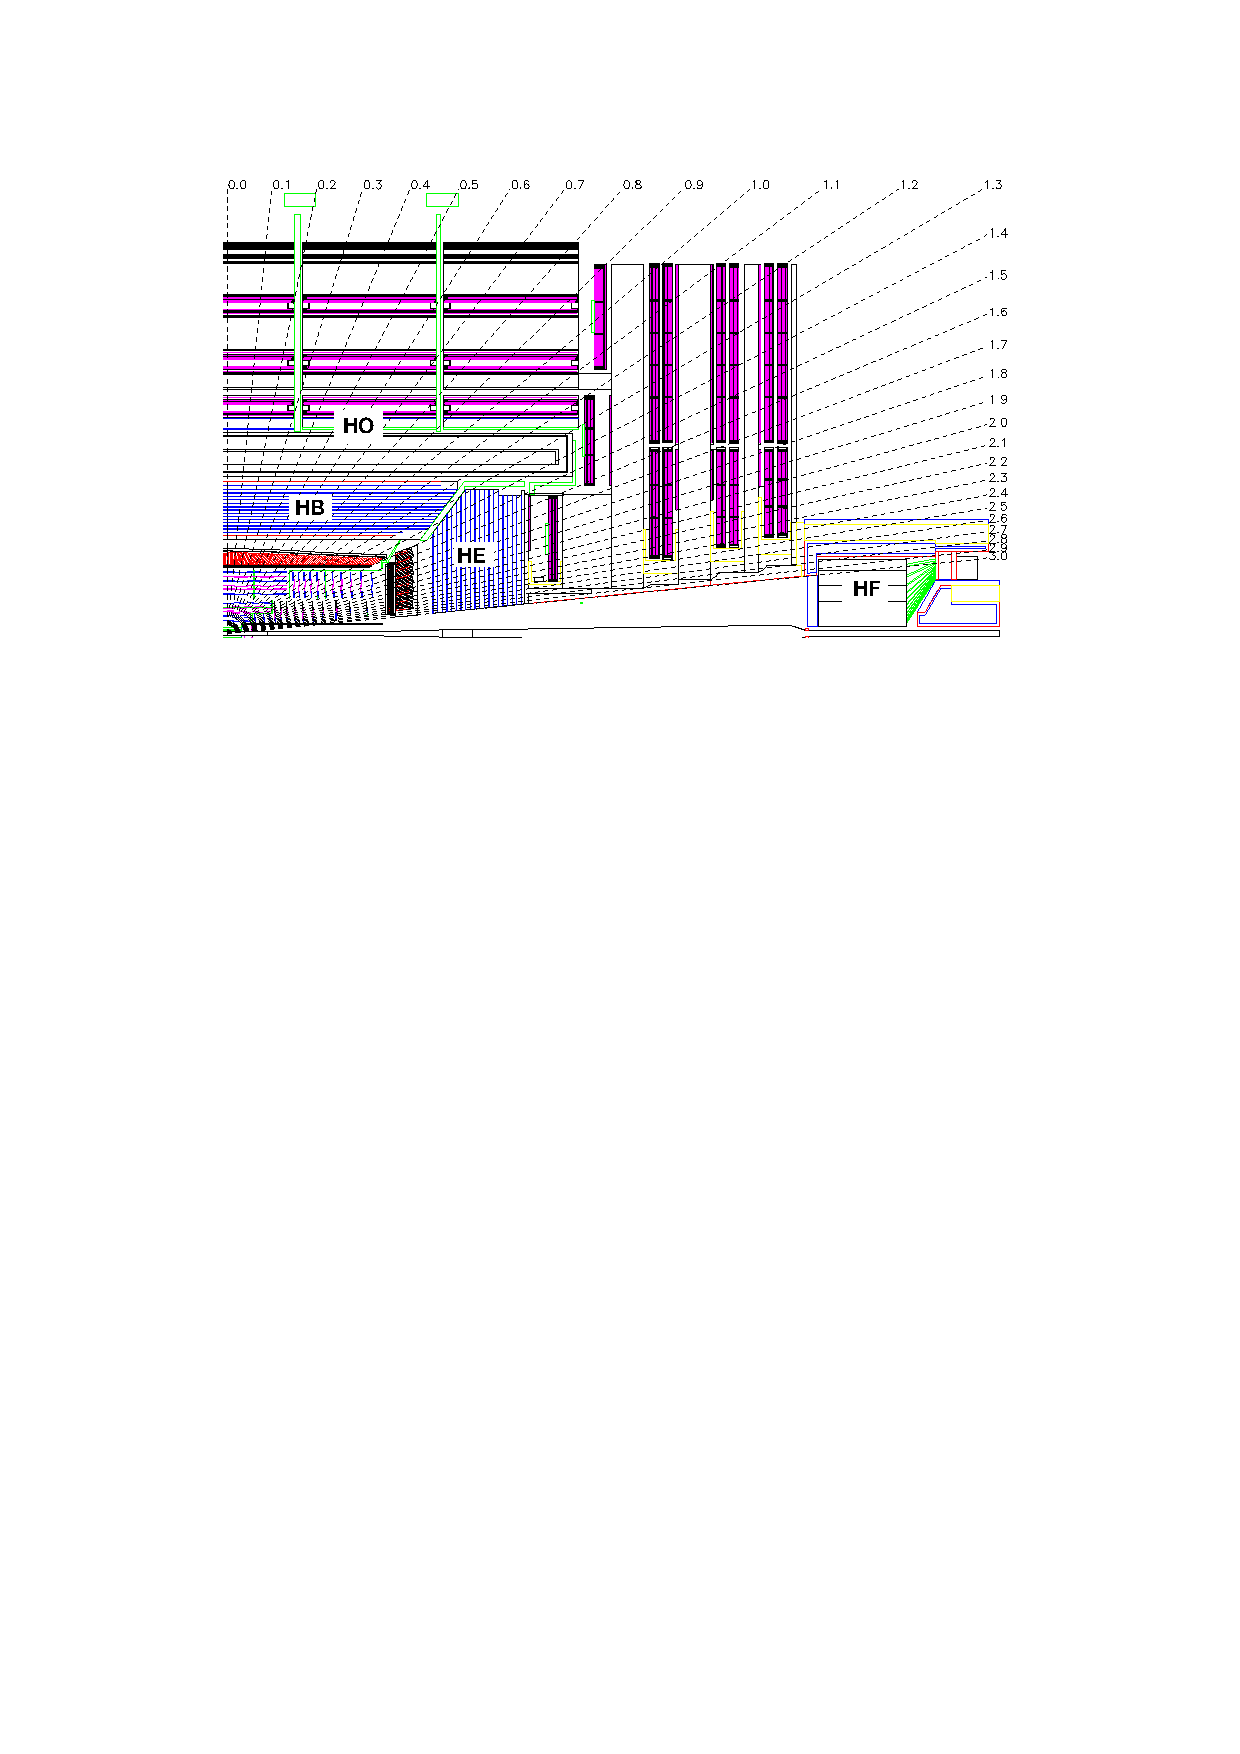
\includegraphics[scale = 1.]{/home/anter/Desktop/Thesis/Figures/edited_cropped_HCAL.pdf}\\
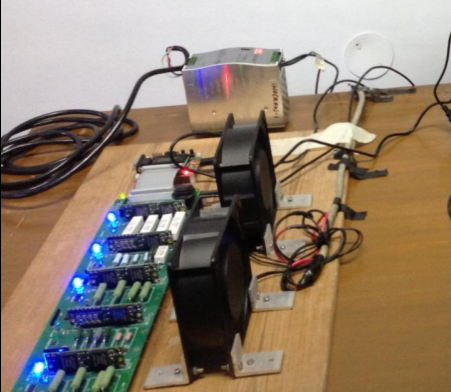
\includegraphics[scale = 0.8]{/home/anter/Desktop/Thesis/Figures/Final/Mezannine_3.png}\\
\vspace*{4mm}
\caption[Longitudinal section of one quarter of the hadronic calorimeter (HCAL) in $r$-$\eta$ plane.]{Longitudinal section of one quarter of the hadronic calorimeter (HCAL) in $r$-$\eta$ plane. It consists of different parts : hadron barrel (HB), hadron outer (HO), hadron endcap (HE) and hadron forward (HF). Taken from \cite{Chatrchyan:2008aa}.}
\label{fig:mez}
\end{center}
\end{figure}

The new sensors and capabilities of
the HCAL will require new ADC (Analog to digital conversion) and
data transmission ASICs (Application-specific integrated circuits).


 The new SiPM system developed will be consisting of two circuit boards,
the Mounting Board (MB) and the Control Board (CB). The array
of 18 SiPMs is mounted on one side of the MB. On the other side a
Peltier cooler is placed to arrange for a constant temperature of the
SiPMs.


\cite{DN}


1. During upgradation of LHC, in HCAL Back-end electronics, the current VME (VERSAbus Memory card) based system was replaced with modern FPGAs and the μTCA (Micro Telecommunications Computing Architecture) based system to process large amount of data. In μTCA, twelve μHTR (HCAL Trigger/Readout) cards will receive the data links from the front-ends, calculate and transmit trigger primitives. A set-up for testing of μHTR cards was installed at Department of Physics, Panjab University, Chandigarh and we successfully tested μHTR cards. 

2. I was deputed to CERN from 9th February, 2015 to 7th May, 2015. I took 2 DQM (Data Quality Monitoring) and 14 DAQ (Data Acquisition) shifts at P5, CMS Experiment site.

3. Also tested uHTR cards at 904 building (Prevessin site in France) and installed them in μTCA crates at CMS P5 site. Tested Power Modules (PM) at 904 (Prevessin site) which will supply power to μTCA crates.

1. Participated in taking runs for Quality Control (QC) analysis remotely as well as at CERN, in which various runs for e.g. LED, Pedestal (Ped), LED_PED_long etc. were taken by the Hadron Outer (HO) group to analyze and study properties of Silicon Photomultipliers (SiPMs) used in replacement to Hybrid Photon Detector (HPD) in the Readout Modules (RMs).

2. Two properties of SiPMs were studied by developing a code to obtain plots which described the variation in SiPM properties for 18 channels of 92 RMs for five different runs, where one run was taken as a reference.

a) Variation in Breakdown Voltage (BV): To study the variation in BV with time, LED_IV runs were considered. The following formula was used to calculate the variation in BV relative to the reference run.
Variation in BV = [BV – BV(ref)]

SiPMs were found to be stable within 50mV.

b) Relative variation in Gain: In order to study relative variation in SiPM Gain, pedestal runs were considered. The variation was then calculated using the formula:
Relative Gain = [Gain – Gain(Ref)]/[Gain(Ref)]

The relative variation for all channels and RMs was found to be within 3%.

This work was presented under the title "MPPC Photon Sensor Operational Experience in CMS" in 16th International Conference on Calorimetry in High Energy Physics "CALOR 2014", which took place from 6-11 April, 2014 at South Campus, Justus Liebeg University Giessen, Germany.

3. As a part of Hadron Calorimeter (HCAL) back-end upgrade, a Micro Telecommunications Computing Architecture (μTCA) based data acquisition system was used in the replacement of VME to account for high energy and luminosity. μTCA consists of twelve HCAL Trigger/Readout (μHTR) cards, capable of receiving the data links from the front-end, calculating and transmitting trigger primitives. In order to test the working of μTCA system:

a) A test stand was installed at Department of Physics, PU to carry out a 39 hours test in order to check the functioning of power mezzanines (PMs), responsible for supplying the power to μHTR cards. Three sets were successfully tested, each set consisting of 5 mezzanines.

b) Tested μHTR cards at 904 building (Prevessin site in France) and installed them in μTCA crates at CMS P5 site. Also tested Power Modules at 904 which supply power to μTCA crates.

c) A set-up for testing of μHTR cards was also installed at Department of Physics, PU.

4. Participated in the installation of Optical Splitters to be used in the Hadron Barrel/Endcap
 (HB/HE) part of HCAL, in which μTCA system is being used in parallel with the VME system.

5. Currently working on the Data Certification of 2016 CMS data in the DQM (Data Quality Monitoring) group of PPD (Physics Data And Monte-Carlo Validation).

